\documentclass[conference,compsoc]{IEEEtran}
\ifCLASSOPTIONcompsoc
  \usepackage[nocompress]{cite}
\else
  \usepackage{cite}
\fi

\ifCLASSINFOpdf
\usepackage[pdftex]{graphicx}
\usepackage{wrapfig}
\graphicspath{ {images/} }
\usepackage[utf8]{inputenc}
  
\else

\fi

\usepackage[cmex10]{amsmath}

\usepackage{lipsum}



\begin{document}

%Probably i can add the name of a specific gesture type from
%a myo pubication 
\title{Gesture to Speech HMI using machine-learning methods and Myo armband}

\author{\IEEEauthorblockN{Vladislav Isaak}
\IEEEauthorblockA{Exia Cesi \\Computer Engineering School,\\
Bordeaux, France.\\ 
2017}
\and
\IEEEauthorblockN{Jérôme Brallet}
\IEEEauthorblockA{Exia Cesi \\Computer Engineering School,\\
Bordeaux, France.\\ 
2017}}
\maketitle


\begin{abstract}
In the 2017 almost everyone heard about incredible results obtained by using machine-learning(ML). For general public, with IT zero knowledge, mass media invented even more impressive word - Neural Networks(NN). However NN represents only a small part of ML domain. And even if NN can show sometimes results that no one expected, there are cases when it's not the best choice. In this parer we'll explore 5 different ML algorithms including a medium complex NN, applied to gesture classification task. Also, we'll pass thought data acquisition step and feature selection process. By the end we will build a gesture recognition system based on most accurate algorithms.


\end{abstract}
\textbf{Keywords:} gesture, text to speech, recognition, feature selection, classification, myo armband, machine learning, svm, lstm, kmeans.

\IEEEpeerreviewmaketitle

\section{Introduction}
The notion of a 'gesture' can have many interpretations. To define some boundaries and for the sake of simplicity, we will consider only gestures performed with left arm. It is simple enough to collects data and, at the same time it will give us a clear idea about limits of our recognition model. A 'one-side' model can also be easily generalized to take in account both, left and right arms. Concerning classification, we will not try to build a real-time classification model. Partially it is due to a temporal nature of our data. When trying to classify gestures we have a time dimension to consider, it's different from static data like images. On the other hand the amount of values per second is around 250. This will have a serious impact on performances of real-time classification. Let's begin by description of a global architecture of our solution.

\section{Technical Approach}
In order to collect and process data we used follows components. First, Myo armband is connected to a Laptop using Bluetooth LE beacon. Laptop runs a special program written in C\#. This software can collect Myo data, pre-process it and send it to a server in Google Cloud. Virtual machine in the cloud has Web Service build with Flask. This service accept HTTP POST requests from Laptop and it inserts received data into NoSQL database - MongoDB. Another software in the cloud is written in Python. It retrieve data from MongoDB, process it in different ways and starts training of ML algorithms. Than it saves obtained models so they can be reused.


\begin{figure}[h]
\caption{Architecture overview}
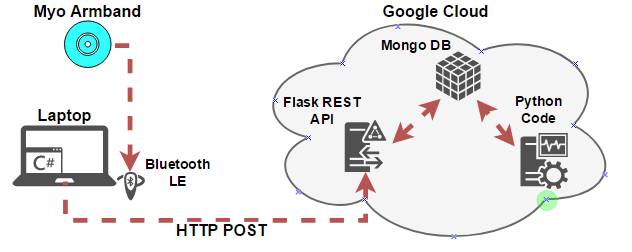
\includegraphics[scale=0.45]{archi}
\centering
\end{figure}

This architecture allow us to control data acquisition process that is performed locally. It also give us enough computational power because all heavy processing is performed on scalable VM in the cloud.  




\section{Data Acquisition}
\subsection{Myo data gathering}

Myo armband provides two main type of information electromyographical data (EMG) and Internal Measurement Unit data (IMU). EMG sensors has eight values in a diapason from -100 to + 100. IMU sensors has 10 values in a diapason from -10 to +10. IMU is a combination of three different measurements - Acceleration(XYZ), Gyroscope(XYZ), Orientation(XYZW).

But when it comes to data collection step, we had to deal with some specific problem. The problem is in how Myo send its data. During experimentation we saw that EMG and IMU are sent in a totally independent manner. So, for example, after 1 second of recording we can obtain 60 IMU entries and 200 EMG entries. Generally EMG data is dent three time more often than IMU data. 

Of course it's difficult to train a classificator with two separate feature sets, so we developped a synchronization algorithm. This algorithm is run afre data recording is over. \begin{wrapfigure}{l}{0.18\textwidth}
    \centering
    \caption{Example of synchronization results}
    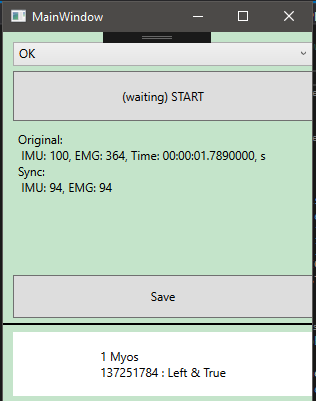
\includegraphics[width=0.17\textwidth]{sync}
\end{wrapfigure} It synchronize IMU and EMG data by looking for a closest timestamps. And at the end we obtain only one feature set with IMU and EMG integrated in it.

After EMG-IMU synchronization some high level features are added to out feature set. We decided to use pitch, roll and yaw to summarize IMU data and Mean Absolute Value(MAV) for EMG data. 

\subsection{Gestures}
To test the ability of out model to recognize gesture we need some samples but distinct gestures that we can use in real world. Those gestures will serve to build a POC for our system and if it work, then we'll increase the number of gestures in our dataset to explore model's limits. We have picked four hand signals from non verbal communication language of Russian Special Purpose Forces (Spetsnaz).
\begin{figure}[h]
\caption{Chosen gestures for a POC}
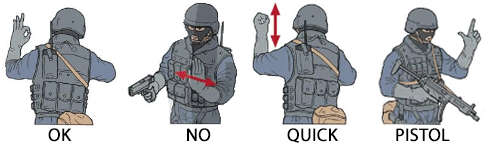
\includegraphics[scale=0.45]{gest}
\centering
\end{figure}


For each gesture we have recorded 20 samples trying to keep them as similar in terms of time as possible. All recorded gesture were saved in the database without any pre-processing except EMG-IMU synchronization using follows format:

\verb|['GestureName': 'NAME',| 

\verb|'Data': [TIME-STEPS x FEATURES]]|

Due to the fact that MongoDB is NoSQL database, we don't need to worry about data structure and data types. Every recording is saved as it is using dociment-like style.

\section{Datasets}
\subsection{Data preparation}
When we retrieve data from the database it is represented like a list of lists of dictionaries. This is an absolutely inappropriate format for any algorithms. So the first step is to convert raw data from MongoDB into a meaningful 4D numpy array with following structure: CLASSES x SAMPLES x FEATURES x TIME-STEPS. Here CLASSES are gestures to recognize. SAMPLES are recordings of a gesture. FEATURES are Myo Data (Acc, Gyro, EMG ...). TIME-STEPS shows evolution of FEATURES from the beginning of gesture to the end.

There is not many algorithms that are able to work with time dimension and most of them are intended to predict time series, not classify them. In this paper, we will try two different approaches to deal with time series - Time series flattening and Featurization. 

\subsection{Time series flattening }
\subsubsection{Temporal scaling}

Before flattening time series we need to normalize them. While each gesture and even each sample has different length we will not be able to put them in to a matrix. It necessary that all time series in our dataset has the same length. We can resample them by applying Fast Fourier Transform. We used and average length as a final signal length.
\subsubsection{Flattening}

Now we can actually obtain a CLASSES x SAMPLES x FEATURES x TIME-STEPS matrix. Then we flatten two last dimensions of this matrix using Fortran-style flattening. It give us a new matrix like this: CLASSES x SAMPLES x ( FEATURES x TIME-STEPS ) with around 1200 features per sample.
\subsection{Featurization}
Another approach consists in summarization of time series using some predefined functions. 

Let's take a feature 'N' as example. Feature 'N' has a time dimension 'T' with 72 time steps. We can describe 'N' buy finding Min, Max, StDev, Mean values of its 'T'. By doing this we can obtain many time independent features from one time dependent.

Now we'll apply this procedure independently to all time series and then flatten the results. It will give us a new matrix CLASSES x SAMPLES x ( FEATURES x FEATURIZED-TIME-STEPS) with around 100 features per sample. 

Those are functions that we used during featurization step: a\textit{mplitude, percent-beyond-1-std, maximum, max-slope, median, median-absolute-deviation, percent-close-to-median, minimum, skew, std, weighted-average}.

\subsection{Spatial scaling}
Even if the variance of our data is not very high, we can perform a spacial scaling. It will bring all values in the dataset to a range from 0 to 1. This method is used sometimes to punish outling values. 

\section{Feature selection}
Not all of features may be useful. But how can we now what features to use. Even if some of them seems useful, in reality they can lower the quality of classification. Also it's not clear if low lever features(ex: 8 EMG values) are better than high level features (ex: EMG Mean Absolute Value). In this step well create multiple Datasets with different features. Then we'll apply basic clusterization method to find are the features that describes data in the most accurate way. 

Finally we obtained multiple datasets with different characteristics. For some of them Time series flattening were used, for others featurization. For some we included spatial scaling. For some datasets we used only high level features, for others only low level. 

When various datasets were ready we used k-means clusterization algorithm to find the most appropriate dataset. K-means is one of the simplest unsupervised learning algorithms. It goal is to find clusters in dataset without any knowledge about data. The only thing it knows is the number of clusters to lok for. Basically, if k-means managed to find right number of distinct cluster that means features in the dataset are good for describe the data.

\subsection{K-means results}
After running all datasets through k-means we have obtained three type of graphs. 
Fist type corresponds to datasets with specially scaled data. For some reason, in those datasets clusters are squeezed and looks like a linear function. 
\begin{figure}[h]
\caption{Dataset with scaled data}
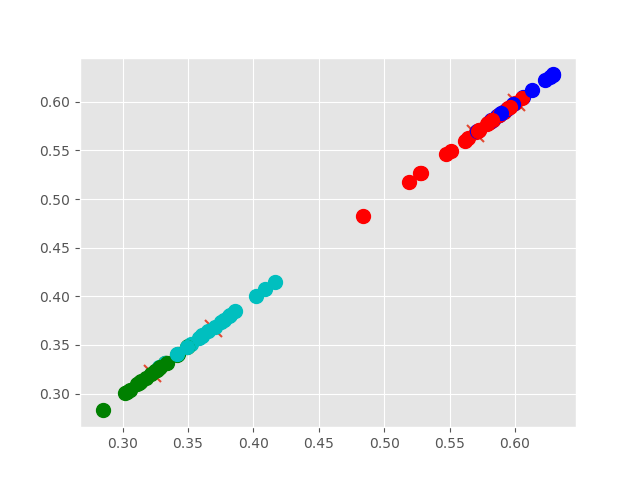
\includegraphics[scale=0.40]{ds1}
\centering
\end{figure}

The second type of graphs contains complete mess and are absolutely unusable. Those corresponds to datasets with flattened time series. It probably du to the overwhelming number of features per sample.

\begin{figure}[h]
\caption{Datasets with flattened time series}
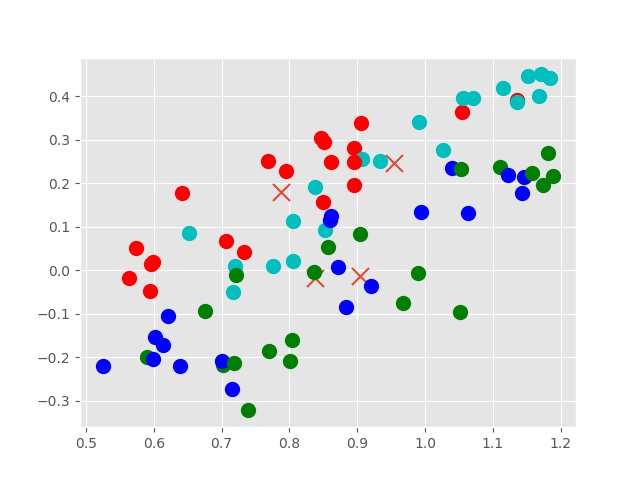
\includegraphics[scale=0.40]{ds2}
\centering
\end{figure}

The third type corresponds to datasets with featurized time series. Here we can observe a surprisingly accurate distinction between 4 clusters corresponding to 4 gesture in our dataset.

\begin{figure}[h]
\caption{Datasets with featurized time series}
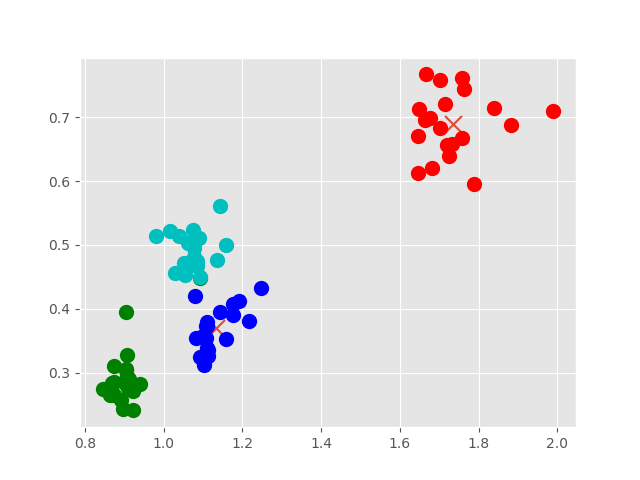
\includegraphics[scale=0.40]{ds3}
\centering
\end{figure}

Obviously featurization is the best way to represent time series so we'll use this dataset to train classification models.

\section{Models}
\subsection{SVM}
\subsection{Naive Bayes}
\subsection{Decision Trees}
\subsection{Deep Neural Network}
\subsection{LSTM}

\section{Tests}
\subsection{Protocol}
There two ways to test this system.
\subsubsection{Observation based}
 First of all we can put on a Myo armband, perform gesture and observe results. In this case we we'll not have any specific metrics but a person will be directly observe the result.
To perform this test method you need to stand strait up with Myo armband on your left hand. Myo must be connected to a specific software that can communicate with trained models. This software has two buttons "Start recording" and "Stop recording". Click "Start recording" and start performing gesture. Click "Stop recording" when gesture is over. Data will be sent to a server and result will be displayed on the screen.
\subsubsection{Data based}
This method is more precise and quantifiable. We can split our dataset in two parts. Training part will represent 80\% of data and it will be used to train classificator. Testing part will represent 20\% data and it will be used after model training is over. Model will be asked to classify data from testing part. Than we will choose a error function to calculate the percentage of how accurate is our model. Also, if the size of dataset is not big enough to split it in two parts, it is possible to use cross-validation method to obtain same accuracy value.
\subsection{Metrics}

For out tests we well be using following accuracy function. 

$ accuracy(y,y') = \dfrac{1}{n_{samples}}\sum_{i=0}^{n_{samples}-1} 1(y'_{i} =y_{i}) $

Here, $y$ is correct classes and $y'$ are model's predictions. This function will return the fraction of correct prediction over $n_{samples}$. The best performance is when the function returns 1. In the worst case it returns 0.

\subsection{Results}

\section{Future work}

\begin{thebibliography}{9}
\bibitem{time_series_comparison} 
Zainal Arief, Indra Adji Sulistijono, Roby Awal Ardiansyah. 
\textit{Comparison of Five Time Series EMG Features Extractions Using Myo Armband}. 
2015 International Electronics Symposium (IES).

\bibitem{gesture_control_capabilities} 
Adam B. Csapo, Árni Kristjánsson, Hunor Nagy, György Wersényi. 
\textit{Evaluation of Human-Myo Gesture Control Capabilities in Continuous Search and Select Operations}. 
7th IEEE International Conference on Cognitive Infocommunications (CogInfoCom 2016) • October 16-18, 2016 • Wrocław, Poland.

\bibitem{posture_and_gesture_recognition} 
Ali Boyali, Naohisa Hashimoto and Osamu Matsumoto. 
\textit{Hand Posture and Gesture Recognition using MYO Armband and Spectral Collaborative Representation based Classification}. 
2015 IEEE 4th Global Conference on Consumer Electronics (GCCE). 

\bibitem{myo_game} 
Karen Yang, David Pan. 
\textit{Myo the Force Be With You}. 
Stanford EE 267, Virtual Reality, Course Report, Instructors: Gordon Wetzstein and Robert Konrad. 

\bibitem{algorithm_for_efficient_hci} 
Ehab H. El-Shazly, Moataz M. Abdelwahab, Atsushi Shimada and Rin-ichiro Taniguchi. 
\textit{Real Time Algorithm for Efficient HCI Employing Features Obtained From MYO Sensor}.
2016 IEEE 59th International Midwest Symposium on Circuits and Systems (MWSCAS), 16-19 October 2016, Abu Dhabi, UAE). 

\bibitem{wavenet} 
Aaron van den Oord, Sander Dieleman, Heiga Zen, Karen Simonyan, Oriol Vinyals, Alex Graves, Nal Kalchbrenner, Andrew Senior, Koray Kavukcuoglu. 
\textit{WAVENET: A GENERATIVE MODEL FOR RAW AUDIO}. 
Google DeepMind, London, UK.

\bibitem{spectre} 
Prajwal Paudyal, Ayan Banerjee, and Sandeep K.S. Gupta. 
\textit{SCEPTRE: a Pervasive, Non-Invasive, and Programmable Gesture Recognition Technology}. 
Arizona State University, Tempe, Arizona). 

\bibitem{sign_language_recognition} 
Hardie Cate, Fahim Dalvi, Zeshan Hussain. 
\textit{Sign Language Recognition using Temporal Classification}. 
December 11, 2015. 

\bibitem{sign_language_recognition} 
R. Langmann. 
\textit{Google Cloud and Analysis of Realtime Process Data}. 
Duesseldorf University of Applied Sciences/Competence Center Automation Duesseldorf (CCAD), Duesseldorf, Germany. 

\bibitem{myo_mocap} 
Yanbin Xu, Chenguang Yang, Peidong Liang, Lijun Zhao and Zhijun Li. 
\textit{Development of a Hybrid Motion Capture Method Using MYO Armband with Application to Teleoperation}. 
Proceedings of 2016 IEEE International Conference on Mechatronics and Automation August 7 - 10, Harbin, China.

\bibitem{lstm1} 
Dong Wu and Mingmin Chi , Member, IEEE. 
\textit{Long Short-Term Memory with Quadratic Connections in Recursive Neural Networks for Representing Compositional Semantics}. 
Proceedings of 2016 IEEE International Conference on Mechatronics and Automation 2016 IEEE.


\end{thebibliography}

\end{document}